%% What Speculative Decoding Costs on a CPU
%%
%% Draft. Build with `make` in this directory; see README.md for the toolchain and for the list of
%% numbers still marked \pending. Every measured figure in this paper carries the context length and
%% the machine state it was taken under, because on the hardware used here a figure without them is
%% not a figure -- see Section~\ref{sec:method}.
\documentclass[conference]{IEEEtran}

\usepackage{cite}
\usepackage{amsmath,amssymb}
\usepackage{graphicx}
\usepackage{booktabs}
\usepackage{xcolor}
\usepackage[hidelinks]{hyperref}
\usepackage{url}

\graphicspath{{../results/figures/}}

% A number that has not been measured yet. Every one of these is listed in README.md.
\newcommand{\pending}[1]{\textcolor{red}{[#1]}}

\begin{document}

\title{What Speculative Decoding Costs on a CPU:\\Measuring the Verification Term}

\author{\IEEEauthorblockN{Aadit Sood}}

\maketitle

\begin{abstract}
The standard speedup model for speculative decoding assumes that verifying $\gamma+1$ draft tokens in
one forward pass costs about as much as generating a single token. On a GPU that is nearly true: the
pass is bound by reading the weights, the weights are read once however many tokens share the pass,
and the extra arithmetic disappears into spare throughput. A CPU has no spare throughput. We replace
the constant with a measured term $v(k)$, the cost of verifying $k$ tokens in one pass relative to an
ordinary step, and report it for a 4-bit Qwen3-4B target with a 4-bit Qwen3-0.6B draft on a six-core
laptop CPU, using an inference engine written from scratch in which a $k$-token verification pass is
bit-identical to $k$ single-token passes. We find $v(k)$ rises with both $k$ and context: $v(2)$ goes
from 1.13 at context 128 to 1.25 at 2048, and $c$, the draft-to-target step ratio, from 0.182 to
0.245. The term is not a correction but the thing that selects the configuration. Assuming $v=1$
predicts $1.79\times$ at $\gamma=3$ where the engine measures $1.06\times$, an error that grows
monotonically from $1.23\times$ at $\gamma=1$ to $1.83\times$ at $\gamma=4$. We then extend the model
from decoding to wall clock with a single term for the prompt pass, which speculative decoding pays
for twice, and show that the extension needs no new free parameter: the draft's prompt pass costs the
same fraction of the target's that its decode step does. The extended model predicts measured
wall-clock speedup to 3.9\% mean absolute error over 29 runs and, unlike the decode-only model,
correctly selects the better of two drafting strategies in all ten cases where they are compared,
including both of the reversals in which a drafter that accepts less than half as often nonetheless
wins the clock.
\end{abstract}

\begin{IEEEkeywords}
speculative decoding, CPU inference, quantization, performance modelling, memory bandwidth
\end{IEEEkeywords}

\section{Introduction}

Speculative decoding~\cite{leviathan2023,chen2023} runs a small draft model $\gamma$ tokens ahead of a
large target model, then verifies all $\gamma+1$ candidate tokens in a single forward pass of the
target. When the draft is right the target emits several tokens for the price of one pass; when it is
wrong the work is discarded. With greedy decoding, or with the standard modified rejection sampling,
the output is identical to what the target alone would have produced, so the technique is a pure
latency optimisation.

Its speedup is conventionally written
\begin{equation}
S(\gamma) = \frac{\tau(\gamma)}{\gamma c + 1},
\qquad
\tau(\gamma) = \frac{1 - \alpha^{\gamma+1}}{1 - \alpha},
\label{eq:classic}
\end{equation}
where $\alpha$ is the per-token acceptance rate and $c$ is the cost of a draft step relative to a
target step. The constant $1$ in the denominator is the verification pass. It encodes the assumption
that checking $\gamma+1$ tokens costs one ordinary step, which holds when the pass is bound by weight
traffic rather than arithmetic.

This paper is about what happens when that assumption fails. On a CPU the weights are still read once
per pass, but the integer multiply--accumulates grow linearly with the number of tokens in the pass,
and on six cores they are not free. The denominator therefore needs a measured term:
\begin{equation}
S_{\text{decode}}(\gamma) = \frac{\tau(\gamma)}{\gamma c + v(\gamma+1) + o},
\qquad
v(k) = \frac{\text{pass}(k)}{\text{pass}(1)},
\label{eq:vk}
\end{equation}
with $o$ a per-round overhead for sampling and bookkeeping.

Our contributions are:
\begin{itemize}
  \item A measurement of $v(k)$ for a realistic target/draft pair on a commodity CPU, across four
        context lengths, showing that $v(k)$ is a function of context and not a constant
        (Section~\ref{sec:vk}).
  \item Evidence that $v(k)$ selects the operating point rather than merely correcting it: the
        classic model~\eqref{eq:classic} chooses a $\gamma$ at which this engine is slower than not
        speculating at all (Section~\ref{sec:gamma}).
  \item An extension of the model from decoding to wall clock with one term for the prompt pass,
        which introduces no new free parameter and which predicts \emph{which drafting strategy
        wins} --- something the decode-only model cannot express (Section~\ref{sec:wall}).
  \item A measurement methodology for a thermally and contention-limited machine, including a
        failure mode we found in our own earlier results: a parameter sweep visited in a fixed order
        cannot distinguish drift from the effect it measures (Section~\ref{sec:method}).
\end{itemize}

\section{Background and Related Work}

Blockwise parallel decoding~\cite{stern2018} established that several tokens can be verified in one
pass. Leviathan et al.~\cite{leviathan2023} and Chen et al.~\cite{chen2023} gave the modern form with
its acceptance-rate analysis and the speedup model in~\eqref{eq:classic}. Subsequent work largely
accepts that model's cost structure and attacks $\alpha$ or $\gamma$: DistillSpec~\cite{zhou2024}
trains the draft to agree with the target, SpecDec++~\cite{huang2024} adapts the candidate length
online, and FR-Spec~\cite{zhao2025} shrinks the drafting vocabulary. Spec-Bench~\cite{xia2024}
standardises evaluation across task categories, and we use its prompts here.

Drafting need not involve a model at all. Prompt-lookup decoding proposes continuations by matching
the recent $n$-gram against earlier text, which costs no model work and therefore no draft prefill ---
a distinction that turns out to decide the wall-clock comparison in Section~\ref{sec:wall}.

Almost all of this literature measures on GPUs, where the $1$ in~\eqref{eq:classic} is a good
approximation. The CPU case has received much less attention, and llama.cpp is the main practical
implementation. We are not aware of prior work that measures the verification cost as a function of
both batch size and context on a CPU and feeds it back into the configuration choice.

The underlying reason the term matters is a roofline argument~\cite{williams2009}: single-token
decoding of a quantized model sits firmly on the bandwidth roof, while a $k$-token verification pass
moves toward the compute roof as $k$ grows. Measuring $v(k)$ is measuring that traverse.

\section{Implementation}

Measuring $v(k)$ requires an engine in which a $k$-token pass is the \emph{same computation} as $k$
single-token passes, or the ratio measures a numerical difference rather than a cost. We therefore
wrote the engine from scratch rather than instrumenting an existing one.

\textbf{Model and formats.} Qwen3-4B~\cite{qwen3} as the target and Qwen3-0.6B as the draft, both
quantized to 4-bit blocks in the Q4\_0 layout used by llama.cpp~\cite{llamacpp} so that a future
comparison is like for like. Weights are memory-mapped; the KV cache is fp16. A PyTorch
reference matches Hugging Face layer by layer, and a quantization twin that fake-quantizes
activations and rounds the KV cache agrees with the engine on 98.9\% of top-1 tokens at 0.023 mean
total variation distance, which is close enough to rank training recipes off-device.

\textbf{Kernels.} The dot-product kernels are AVX2/FMA/F16C at compile time, with an AVX-VNNI path
selected at run time via \texttt{\_mm256\_dpbusd\_avx\_epi32}. Eight 4-bit blocks share one set of
fp16 scale conversions; the sign trick is replaced by the offset identity $\sum (q-z)x = \sum qx - z
\sum x$ with a precomputed per-block integer; and one 32-byte load covers two blocks whose nibbles
are already adjacent.

\textbf{Bit-exactness.} The same templated kernel serves single tokens, verification and prompt
processing, so the summation order is identical. Attention sums positions in fixed 256-position
chunks, making the order a function of position rather than of how many tokens are in flight. A
$k$-token pass is tested bit-identical to $k$ single-token passes for $k = 1 \ldots 13$ and across
chunk and tile boundaries, and greedy speculative output matches plain greedy decoding token for
token. The round loop, sampling, the acceptance rule and the seeded RNG are all in C++, so no
interpreter overhead enters a timing. The suite is 906 tests.

\section{Methodology}
\label{sec:method}

The measurements in this paper were taken on an Intel Core i7-13620H (6 performance cores, 4
efficiency cores, 16\,GB DDR4-3200) running Windows. A laptop of this kind is a poor instrument, and
most of the methodology here exists to make it a usable one.

\textbf{Everything is relative to a measured ceiling.} Read bandwidth over the six performance cores
measures 40.19\,GB/s against a theoretical 51.2, which caps single-token decoding at 17.8 tokens per
second for a 2.26\,GB weight set. Absolute token rates are reported as a share of that ceiling. We
measure the ceiling with a read-only kernel rather than with STREAM~\cite{mccalpin}, whose copy and
triad kernels include stores and so understate what matters here: inference only reads weights.

\textbf{Conditions are recorded at both ends of a session.} A dispatch-overhead probe is read exactly
once in a fresh process --- it builds a thread pool and runs thousands of empty all-core barriers, so
reading it twice measures the heat the first read produced. For the session reported here, dispatch
read 1.474\,$\mu$s at the start and 1.192 at the end, and read bandwidth 40.19 and 40.14\,GB/s: a
0.12\% drift across eight $v(k)$ runs, eight Spec-Bench runs, two per-stage sweeps and 906 tests. All
figures in this paper come from that single session.

\textbf{Comparisons are made inside one process, with variants alternating.} The same unchanged
binary has produced token rates spanning 15\% across four consecutive runs on this machine, so any
A/B that runs variant A to completion and then variant B hands B a hotter machine.

\textbf{A sweep must not visit its parameter in a fixed order.} This is the methodological finding we
consider most transferable, because we failed it ourselves. An earlier $\gamma$ sweep of ours ran
$\gamma = 1,2,3,4$ ascending and back to back, nine minutes for four runs with no cooldown, and
produced decode speedups declining monotonically at $1.201, 1.007, 0.951, 0.882$. The decline looked
like the effect the model predicts, and so went unquestioned. Re-measured with each $\gamma$ visited
in two different orders, $\gamma=1$ reproduces to within 1.6\% while $\gamma=2$ reads 19.1\% higher,
$\gamma=3$ 11.6\% higher and $\gamma=4$ 11.3\% higher. In each pass of the re-measurement, whichever
$\gamma$ ran first won that pass. A monotonic drift is indistinguishable from a monotonic effect, and
agreement with theory is not evidence that the measurement was sound.

Accordingly, every sweep reported below visits its parameter in two different orders, and we report
the average of the two passes along with their spread.

\section{Results}

\subsection{The kernel is at the hardware's limit}

Before any of the speculative-decoding results can mean anything, the engine has to be fast enough
that it is measuring hardware rather than its own inefficiency. Single-token decoding of the 4-bit
4B runs at 72.6\,ms per token, 13.8 tokens per second, which is 77.5\% of the measured bandwidth
ceiling. The $k$-token kernel reaches 95--105\% of the AVX-VNNI issue peak for $k \geq 4$ at six
threads --- 0.030 issue slots per multiply--accumulate where a pure \texttt{dpbusd} stream is 0.031 ---
so the verification pass is issue-bound, not stalled.

Two honest qualifications. First, an earlier session measured the same step at 64.1\,ms, 15.6 tokens
per second and 88.7\% of a slightly lower ceiling, corroborated there by two independent harnesses
agreeing to 0.05\%. The 13\% difference is reproducible and we cannot presently explain it: it is not
bandwidth, which is higher now; not clock, since the per-round overhead $o$ is an absolute cost of
non-streaming work and did not move; and not source, since rebuilding the earlier commit with the
same compiler and flags and alternating it against the current one inside a single process gives a
ratio of 0.975. It is spread across the weight-streaming stages with no single stage responsible.
Second, we deliberately do not report a llama.cpp comparison. A relative figure is only as
informative as the program it is relative to, and establishing that llama.cpp is running
bit-identical weights --- the same model, the same block quantization, the same numbers --- is
difficult enough that a comparison we could not fully defend would be worse than none. The absolute
argument is also the stronger one: that the engine sits within a few percent of what the hardware can
do bounds how much faster \emph{any} implementation could be, which no pairwise comparison does.

\subsection{$v(k)$ is a function of context}
\label{sec:vk}

Table~\ref{tab:vk} gives $v(k)$, $c$ and $o$ at four context lengths, each the average of two
shuffled passes.

\begin{table}[t]
\caption{Verification cost $v(k)$, draft ratio $c$ and per-round overhead $o$, by context. Average of
two passes taken in different orders.}
\label{tab:vk}
\centering
\begin{tabular}{@{}rrrrrrr@{}}
\toprule
context & $v(2)$ & $v(3)$ & $v(4)$ & $v(5)$ & $c$ & $o$ \\
\midrule
128  & 1.125 & 1.350 & 1.624 & 1.936 & 0.182 & 0.0072 \\
512  & 1.206 & 1.518 & 1.919 & 2.314 & 0.208 & 0.0087 \\
1024 & 1.155 & 1.368 & 1.664 & 1.972 & 0.209 & 0.0069 \\
2048 & 1.245 & 1.696 & 2.147 & 2.607 & 0.245 & 0.0073 \\
\bottomrule
\end{tabular}
\end{table}

\begin{figure}[t]
\centering
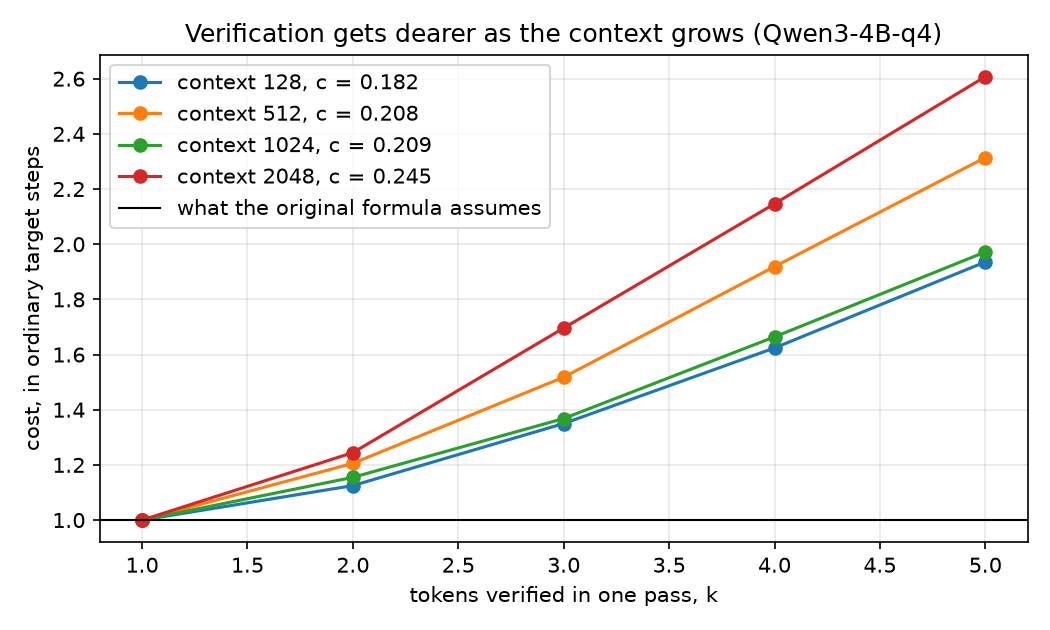
\includegraphics[width=\columnwidth]{vk_by_context_Qwen3-4B-q4.png}
\caption{$v(k)$ at four context lengths, with the line the classic model assumes drawn at 1.0. Each
curve is the average of two passes taken in different orders. The gap between the curves and that
line is the term this paper measures; the gap between the curves is why one number for it is not
enough.}
\label{fig:vk}
\end{figure}

Two tokens cost 1.13--1.25 ordinary steps rather than 1, and five cost 1.9--2.6. The term the classic
model sets to unity is therefore wrong by 13--25\% at $k=2$ and by a factor of two or more at $k=5$.
Figure~\ref{fig:vk} shows the shape: $v(k)$ rises with $k$ at every context, and the whole family
shifts upward as context grows.

The mechanism is that the KV cache is read \emph{per token of the pass}, not once per pass. Weight
traffic is shared across the tokens in a verification pass; attention over the cache is not. So the
part of a pass that $k$ tokens cannot share grows with context, and $v(k)$ grows with it. The same
mechanism drives $c$: the draft's KV cache is nearly as large as the target's while its weights are
about a seventh the size, so the draft becomes relatively more expensive as context grows, which is
what the $c$ column shows.

We are more confident in the direction than the magnitude. $c$ is monotonic in context in every pass
we have taken, in this session and in two earlier ones. The magnitude of $v(2)$'s context dependence
is not pinned: the two passes of this session read spreads of $1.04\times$ and $1.18\times$ across the
same four contexts, so long-context $v(k)$ is the noisy half of the table. A second machine would
settle this \pending{second-machine replication}.

\subsection{$v(k)$ selects $\gamma$; assuming $v=1$ selects wrong}
\label{sec:gamma}

Table~\ref{tab:gamma} gives the measured sweep against both models.

\begin{table}[t]
\caption{Measured speedup by $\gamma$, against the model with measured $v(k)$ and the classic model
with $v = 1$. Each $\gamma$ visited in two orders; decode figures are the average.}
\label{tab:gamma}
\centering
\begin{tabular}{@{}rrrrrr@{}}
\toprule
& \multicolumn{2}{c}{measured} & \multicolumn{2}{c}{predicted (decode)} & \\
\cmidrule(lr){2-3}\cmidrule(lr){4-5}
$\gamma$ & decode & wall & with $v(k)$ & with $v=1$ & $v=1$ error \\
\midrule
1 & 1.193 & \textbf{1.073} & 1.243 & 1.464 & $1.23\times$ \\
2 & 1.200 & 0.986 & 1.231 & 1.689 & $1.41\times$ \\
3 & 1.062 & 0.951 & 1.138 & 1.787 & $1.68\times$ \\
4 & 0.982 & 0.844 & 1.043 & 1.796 & $1.83\times$ \\
\bottomrule
\end{tabular}
\end{table}

Measured acceptance is $\alpha = 0.768, 0.781, 0.789, 0.789$ for $\gamma = 1 \ldots 4$. The model
with measured $v(k)$ predicts the decode column to 5.0\% mean absolute error at context 512 and 5.6\%
at 2048. The classic model overshoots by $1.23\times$ at $\gamma=1$, and the error grows monotonically
to $1.83\times$ at $\gamma=4$: it predicts $1.79\times$ at $\gamma=3$ where the engine measures
$1.06\times$ on decoding and $0.95\times$ on the clock, which is slower than not speculating.

The practical consequence is the selection, not the correction. $\gamma=1$ is the best available
choice, and it is the choice the measured model makes. The classic model's maximum is at $\gamma=3$,
where this engine loses.

\begin{figure}[t]
\centering
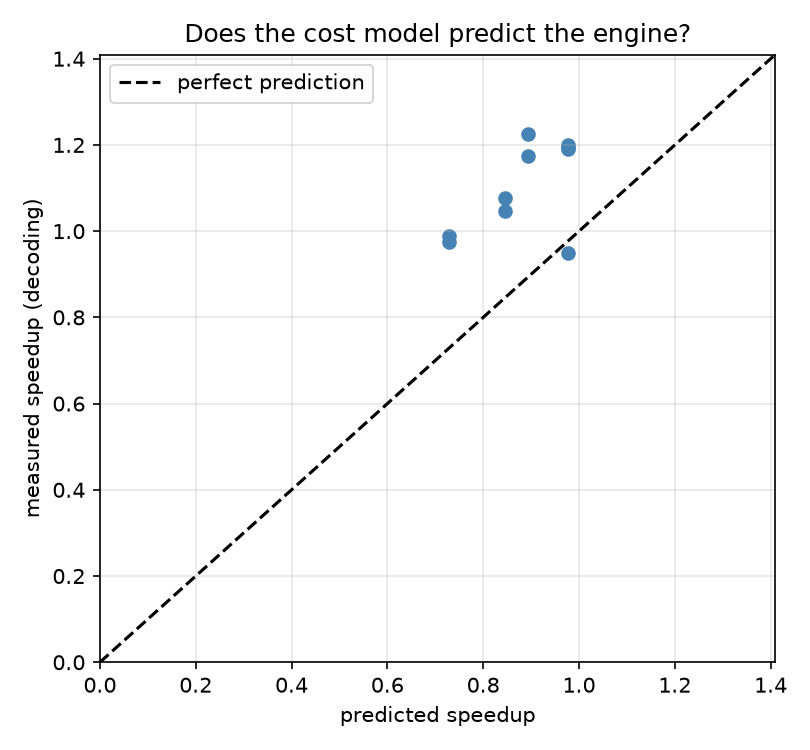
\includegraphics[width=\columnwidth]{predicted_vs_measured.png}
\caption{Predicted against measured decode speedup, over the configurations measured in this
session. Points on the diagonal are exact predictions.}
\label{fig:pred}
\end{figure}

Figure~\ref{fig:pred} plots the predictions against the measurements across configurations.

Two details worth keeping. On \emph{decoding}, $\gamma=1$ and $\gamma=2$ are tied --- 1.193 against
1.200, a 0.6\% gap against a 4.4\% run-to-run spread --- and the decline does not begin until
$\gamma=3$. It is wall clock that separates them, by 8.9\%, for the reason the next section gives.
And confidence-based early stopping is what makes a larger $\gamma$ survivable: plain speculation
falls below parity on the clock at $\gamma=2$ (0.986) where early stopping holds 1.049 at $\gamma=2$
and 1.011 at $\gamma=3$.

\subsection{From decoding to wall clock}
\label{sec:wall}

Equation~\eqref{eq:vk} describes rounds. It says nothing about the prompt pass, which is 27--88\% of
the clock in these runs and which speculative decoding pays for \emph{twice}, once into each model's
KV cache. The number a user experiences is therefore outside the model, and so is the question of
which drafting strategy to use.

Greedy speculative decoding emits exactly the tokens the target would, so both runs generate the same
$N$ tokens and only the rates differ. Writing $P$ for the prompt pass, $D$ for the decode phase,
$f = P_t/(P_t + D_t)$ for the target's prefill share and $k = P_d/P_t$ for the draft's prompt pass
relative to the target's,
\begin{equation}
S_{\text{wall}} = \frac{1}{(1+k)\,f + (1-f)\,/\,S_{\text{decode}}}.
\label{eq:wall}
\end{equation}

The useful property of~\eqref{eq:wall} is that $k$ is not a new free parameter. Measured directly from
recorded prefill times, $k = -0.005$ (range $-0.027$ to $0.013$) for prompt lookup, which is zero
within noise as its structure demands since it runs no model; and $k = 0.183$ (range $0.152$ to
$0.236$) for the model draft, against $c = 0.182$ at context 128 rising to $0.245$ at 2048. The
draft's prompt pass costs about the same fraction of the target's that its decode step does, so
\eqref{eq:wall} is evaluable from quantities~\eqref{eq:vk} already needs.

Scored against 29 method-runs --- four $\gamma$ values in two passes, plus the short- and long-prompt
sets --- \eqref{eq:wall} gives 3.9\% mean absolute error (2.6\% for lookup, 3.1\% for early stopping,
6.0\% for plain speculation; worst case 12.7\%). At $\gamma=1$ it predicts plain speculation to
$+0.1\%$ and $-0.1\%$ in the two passes.

What it buys is the selection of a drafting strategy, which the decode-only model cannot express at
all: prompt lookup loses on decoding in \emph{every} run measured here, so a decode-only reading ranks
it last everywhere. Table~\ref{tab:reversal} shows it winning the clock at two of the three operating
points, and~\eqref{eq:wall} predicting the winner at all of them.

The three points come from two prompt sets, not three: the four-category rows and the short row are
the \emph{same eight prompts} at different generation lengths (152 against 54 tokens a turn), which
is a legitimate way to vary $f$ --- the prefill share is what the model claims decides this --- but it
is a weaker test than three distinct prompt distributions would be, and we say so in
Section~\ref{sec:limits}.

\begin{table}[t]
\caption{Wall-clock speedup at $\gamma=1$ for a model draft and for prompt lookup, against the
break-even prefill share $f^\star$ from~\eqref{eq:wall}.}
\label{tab:reversal}
\centering
\begin{tabular}{@{}lrrrrl@{}}
\toprule
prompt set & $f$ & lookup & model & $f^\star$ & wins \\
\midrule
four-category, A & 0.270 & 1.015 & \textbf{1.074} & 0.440 & model \\
four-category, B & 0.275 & 1.026 & \textbf{1.072} & 0.404 & model \\
short            & 0.450 & \textbf{1.117} & 1.072 & 0.442 & lookup \\
long             & 0.875 & \textbf{0.972} & 0.818 & n/a & lookup \\
\bottomrule
\end{tabular}
\end{table}

Setting the two predictions equal gives the break-even share at which a zero-cost drafter overtakes a
model draft,
\begin{equation}
f^\star = \frac{1/S_L - 1/S_M}{1/S_L - 1/S_M + k},
\label{eq:breakeven}
\end{equation}
and~\eqref{eq:breakeven} depends on both decode speedups, and so on the workload's acceptance rate;
it is a per-set quantity, not a constant. The short set is the sharp test: its measured prefill share sits 0.008
\emph{above} its own break-even, and lookup does win there. On the long set the question does not
arise, because lookup is already ahead on decoding and so has no second prompt pass to repay.

The rule this gives a practitioner is: measure your prefill share, and above roughly 0.4 prefer a
drafter that needs no prompt pass of its own --- even though, at $\alpha$ between 0.088 and 0.431
against the model draft's 0.768, it accepts less than half as often.

\subsection{Where the time goes}

Table~\ref{tab:stages} breaks a decode step into stages at two contexts. Attention is the only stage
whose cost depends on context, and it is the stage that a rewrite of the access pattern improved by
$1.27\times$ at context 128 rising to $2.15\times$ at 2048. The whole step improved $0.86\times$ at
2048 while \emph{regressing} $1.04\times$ at 128, which is the same trade the $v(k)$ table describes
from the other direction.

\begin{table}[t]
\caption{Per-stage cost of one decode step, ms per token, best of two shuffled sweeps.}
\label{tab:stages}
\centering
\begin{tabular}{@{}lrrr@{}}
\toprule
stage & ctx 128 & ctx 2048 & prior shape, ctx 2048 \\
\midrule
qkv       & 13.21 & 13.57 & 13.76 \\
attention & 1.18  & 12.49 & 26.88 \\
attn\_out & 6.57  & 6.56  & 6.97 \\
gate\_up  & 30.76 & 31.03 & 29.91 \\
ffn\_down & 15.29 & 15.25 & 14.79 \\
output    & 6.29  & 6.21  & 6.67 \\
\midrule
step      & 73.29 & 85.11 & 98.97 \\
\bottomrule
\end{tabular}
\end{table}

\section{Limitations}
\label{sec:limits}

\textbf{A small evaluation.} The Spec-Bench subset used here is eight prompts over four categories
(ten turns, 1520 generated tokens) plus two long-prompt questions, against the benchmark's 480
questions. The wall-clock model's strategy selection is validated at three operating points drawn
from two prompt sets, and eight of its ten correct predictions are the same eight prompts at
different $\gamma$, so they are not independent samples. The mechanism behind~\eqref{eq:wall} rests
on ten independent measurements of $k$ and is solid; the strategy-selection claim needs the full
benchmark \pending{full Spec-Bench evaluation}.

\textbf{One machine.} Every number here comes from one laptop. $v(k)$'s shape should depend on the
ratio of memory bandwidth to arithmetic throughput, and a machine with more bandwidth per core should
show a \emph{steeper} $v(k)$; that is a falsifiable prediction we have not yet tested
\pending{second-machine replication}.

\textbf{No external baseline, by choice.} We compare the engine against measured hardware limits
rather than against another implementation. This is a deliberate decision rather than an omission:
a relative number requires establishing that the other program runs bit-identical weights, and a
comparison we could not fully defend would be weaker evidence than the absolute bound. A reader who
wants the relative figure will not find it here.

\textbf{No distilled draft.} The draft is an off-the-shelf Qwen3-0.6B. Our own model, evaluated at the
context the engine runs at, puts distillation to $\alpha = 0.85$ at about $+0.08\times$ on decoding,
and the crossover at which two guesses beat one falls inside reach at 0.818 (context 512) and 0.730
(context 1024) against the measured 0.768 --- but $\gamma=2$ trails $\gamma=1$ by 8.9\% on the clock
for a reason no amount of $\alpha$ touches \pending{distilled draft}.

\textbf{Unexplained absolute shift.} The 13\% step-time difference between sessions noted in
Section~\ref{sec:method} is reproducible and unexplained. It does not affect $v(k)$, $c$ or $o$, all
of which are ratios and all of which reproduce, nor the speedup figures, which are ratios measured
within a run. It is, however, more constrained than a single number suggests. Re-running the
identical prompts through the prompt pass --- a batch-16, compute-heavy phase, unlike the
bandwidth-bound single-token step --- gives $1.143\times$, against $1.133\times$ for the decode step.
Meanwhile $o$, which is pure non-model work, is unchanged at $1.008\times$, and the synthetic
read-bandwidth kernel is \emph{faster} at $1.011\times$. So all model work slowed by the same
$\approx 14\%$ while non-model work on the same cores did not, which rules out a clock or a
scheduling effect and rules out raw sequential bandwidth. A page-locality or TLB explanation would
fit all four observations --- the model walks 2.26\,GB of scattered tensors where the bandwidth probe
streams one contiguous gigabyte --- but we have not tested it and record it only as the first
hypothesis consistent with the constraints.

\textbf{Greedy only.} All speedups are greedy. The sampling path is implemented and tested against the
target's distribution, but the sweeps reported here are at temperature zero.

\section{Conclusion}

The constant that the standard speculative-decoding model puts in its denominator is a statement about
hardware, and on a CPU it is false. Replacing it with a measured $v(k)$ changes not the precision of
the estimate but the configuration it selects: the classic model's optimum is a setting at which this
engine runs slower than no speculation at all. $v(k)$ is moreover a function of context, so a single
measured number is not enough either --- it has to be measured at the context being served.

Extending the model to wall clock requires one further term, for a prompt pass that speculative
decoding pays for twice, and that term costs nothing to obtain because the draft's prompt pass is the
same fraction of the target's as its decode step. With it, the model predicts what a user actually
waits for, and answers a question the decode-only form cannot pose: whether to draft with a model at
all.

\section*{Artifacts}

The engine, the measurement scripts, the stored results with their machine conditions, and the test
suite are available at \pending{repository URL}; a tagged release with a DOI will accompany
publication \pending{Zenodo DOI}.

\bibliographystyle{IEEEtran}
\bibliography{refs}

\end{document}
